\documentclass{article}
\usepackage{graphicx} % Required for inserting images
\usepackage{listings}
\usepackage[english]{babel}
\usepackage[utf8x]{inputenc}
\usepackage[T1]{fontenc}
\usepackage{subcaption}
%% Sets page size and margins
\usepackage[a4paper,top=3cm,bottom=2cm,left=3cm,right=3cm,marginparwidth=1.75cm]{geometry}

\usepackage{amsmath, amssymb}
\usepackage{url} % for \url command

\usepackage{xcolor}
\usepackage[algcompatible]{algorithmicx}
\usepackage[linesnumbered,ruled,vlined]{algorithm2e}
%\setlist{topsep=4pt, itemsep=4pt, partopsep=2pt, parsep=2pt}
\setlength{\parindent}{1.5em}
\setlength{\parskip}{0.5em}

\usepackage{graphicx}

\usepackage{listings}
\usepackage{needspace}
 %\usepackage{algorithm}
%\usepackage{algpseudocode}
\usepackage{xcolor}
\definecolor{mizuasagi}{RGB}{102, 186, 183}
\definecolor{kuchiba}{RGB}{226, 148, 59}
\definecolor{sabiseiji}{RGB}{134, 166, 151}
\definecolor{ouchi}{RGB}{155, 144, 194}
\definecolor{dkgreen}{rgb}{0,0.4,0}
\definecolor{gray}{rgb}{0.5,0.5,0.5}
\definecolor{mauve}{rgb}{0.58,0,0.82}
\definecolor{orange}{rgb}{1,0.3,0.15}
\definecolor{codegreen}{rgb}{0,0.6,0}
\definecolor{codegray}{rgb}{0.5,0.5,0.5}
\definecolor{codepurple}{rgb}{0.58,0,0.82}
\definecolor{backcolour}{rgb}{0.96,0.97,0.98}
\lstdefinestyle{mystyle}{
  backgroundcolor=\color{white},
  commentstyle=\color{sabiseiji},
  keywordstyle=\color{dkgreen},
  numberstyle=\tiny\color{codegray},
  stringstyle=\color{kuchiba},
  basicstyle={\footnotesize\ttfamily},
  breakatwhitespace=false,
  breaklines=true,
  captionpos=b,
  keepspaces=true,                 
  numbers=none,                    
  numbersep=5pt,                  
  showspaces=false,                
  showstringspaces=false,
  showtabs=false,                  
  tabsize=2
}
\lstset{style=mystyle}
\lstset{language=python}
\usepackage{scrextend}
\usepackage{amsmath,amsthm,amsfonts,amssymb,amscd}
\usepackage{titlesec} % For custom sectioning like \subsubsubsection
\titleclass{\subsubsubsection}{straight}[\subsubsection]
\newcounter{subsubsubsection}[subsubsection]
\renewcommand\thesubsubsubsection{\thesubsubsection.\arabic{subsubsubsection}}
\titleformat{\subsubsubsection}
  {\normalfont\normalsize\bfseries}{\thesubsubsubsection}{1em}{}
\titlespacing*{\subsubsubsection}
  {0pt}{3.25ex plus 1ex minus .2ex}{1.5ex plus .2ex}

\usepackage{multirow,booktabs}
\usepackage{fullpage}
\usepackage{lastpage}
\usepackage{braket}
\DeclareMathOperator{\Tr}{Tr}
%\usepackage{stix}
\usepackage{hyperref}
\usepackage[table]{xcolor}
\definecolor{black}{rgb}{0.0,0.0,1}
\hypersetup{colorlinks,breaklinks,
            linkcolor=black,urlcolor=black,
            anchorcolor=black,citecolor=black}
\usepackage{fancyhdr}
\usepackage{mathrsfs}
\usepackage{wrapfig}
\usepackage{tabularx}
\usepackage{setspace}
\usepackage{calc}

\usepackage[linesnumbered,ruled,vlined]{algorithm2e}

\usepackage{multicol}
\usepackage{cancel}
\usepackage[retainorgcmds]{IEEEtrantools}
\usepackage{empheq}
\usepackage{framed}
\usepackage[most]{tcolorbox}
\usepackage{xcolor}
\colorlet{shadecolor}{orange!15}
\parindent 0in
\parskip 0pt
\geometry{margin=1in, headsep=0.25in}
\theoremstyle{definition}
\newtheorem{defn}{Definition}
\newtheorem{reg}{Rule}
\newtheorem{exer}{Exercise}
\newtheorem{note}{Note}
\usepackage{setspace}
\usepackage{minitoc}
\usetikzlibrary{snakes}
\usetikzlibrary{matrix,arrows}
\usepackage{braket}
\usepackage{amsmath}
\usepackage{soul}

\usepackage{algorithm}
\usepackage{algpseudocode}

\usepackage[ruled,vlined]{algorithm2e}
\usepackage{amsmath,amssymb}

% Compact algorithm style (single-page friendly)
\SetAlgoNoLine
\SetAlgoNoEnd
\DontPrintSemicolon
\SetAlFnt{\small}
\SetKwInput{KwInput}{Input}
\SetKwInput{KwOutput}{Output}
\SetKw{KwInit}{Initialize}
\SetKwFor{For}{for}{do}{end}
\SetKwFor{ForEach}{for each}{do}{end}
\SetKwFor{While}{while}{do}{end}
\SetKw{Return}{return}
\usepackage[colorlinks=true, urlcolor=blue]{hyperref}




\usepackage{listings}
\usepackage{color} % Needed for coloring

% Define MATLAB style
\definecolor{MatlabBlue}{rgb}{0.0, 0.0, 0.5}
\definecolor{MatlabGreen}{rgb}{0.0, 0.5, 0.0}
\definecolor{MatlabRed}{rgb}{0.5, 0.0, 0.0}

\lstset{
    language=Matlab,                  % Set the language to MATLAB
    basicstyle=\small\ttfamily,       % Font size and family
    commentstyle=\color{MatlabGreen}\itshape, % Comments in green and italics
    keywordstyle=\color{MatlabBlue}\bfseries,  % Keywords in blue and bold
    stringstyle=\color{MatlabRed},    % Strings (text in quotes) in red
    numbers=left,                     % Line numbers on the left
    numberstyle=\tiny\color{gray},    % Style for line numbers
    stepnumber=1,                     % Step every line
    showspaces=false,                 % Don't show spaces
    showtabs=false,                   % Don't show tabs
    frame=single,                     % Add a box frame around the code
    tabsize=4,                        % Default tab size
    breaklines=true,                  % Wrap long lines
    captionpos=b,                     % Caption position at the bottom
    morekeywords={var, function, end, classdef, properties, methods, global}, % Add common MATLAB keywords
}


\thispagestyle{empty}
\setlength{\parindent}{1em}
\setlength{\parskip}{1em}
\renewcommand{\baselinestretch}{1}



\begin{document}
\begin{titlepage}
    \centering

    {\Huge \textbf{EE 475 Project Report}}\\[3.5cm] % Title made larger


{\Huge \textbf {Optimization-Based Approach to Blind Image Deblurring Using Dictionary Learning}}\\[3.5cm] % Title made larger

    \begin{tabular}{c}
        \Large \textbf{Efe Karakoca (2021401189)} \\[0.5cm] % added spacing between authors
        \Large \textbf{Taha Berk Koç (2021401150)} \\
    \end{tabular}\\[3 cm]

    {\large Introduction to Image Processing | EE 475}\\[0.5cm]

    {\large Boğaziçi University}\\[1cm]

    {\large Fall 2025}

    \vfill

    \begingroup
    \renewcommand\thefootnote{\roman{footnote}}
    \footnotetext{The authors contributed equally to this work.}
    \endgroup

\end{titlepage}


\section{Introduction}



Image deblurring is concerned with various aspects of daily life ranging from daily photography to the medical imaging. Blur can stem from many sources such as measurement equipment (e.g. de-focus blur) or the motion during the exposure time. In order to address this imaging problem, a plethora of methods have been proposed including both classical~\cite{ClassicBlur} and deep-learning based methods~\cite{DeepBlur}. Either classical or deep-learning based methods, many of existing studies rely on harnessing the statistical properties of the image and try to address this inverse problem using Bayesian approaches. The blur which is actuated on the image is usually modeled with the convolution $y=x * h+n$ where $x$ is the clear image, $h$ is the blur kernel, $n$ denotes the noise, which eventually results in the blurred-noisy output $y$. When both the hidden $x$ and the kernel $h$ is unknown, one of the most common way to find the optimal solution is to make use of MAP approach, trying to optimize the posterior distribution:



$$
\begin{aligned}
\left(x^*, h^*\right) & =\underset{x, h}{\operatorname{argmax}} p(x, h \mid y) \\
& =\underset{x, h}{\operatorname{argmax}} p(y \mid x, h) p(x) p(h)
\end{aligned}
$$


However, as Levin \cite{Levin-deblur} mentions, $x=y$, $h=\delta$ solution is collapsed as a trivial one and no de-blurring occurs. To prevent this, we need to adjust the objective function so that this trivial solution is avoided. 


The purpose of the project is to devise an algorithm that de-blurs the blurry image and obtain its clear version without having to know the blur kernel.
The algorithm we have developed is based on initially estimating the blur kernel by learning the distribution of the kernel space and sampling from its posterior distribution, to initiate the multi-scale kernel estimation based on the proposition of Cho and Lee \cite{cho-fast}. 


In order to better make use of the large dataset (whose details are mentioned in the Materials section), we learn a dictionary from the patches of clear images, which is claimed to represent the space where the clear images reside. This dictionary is then utilized to solve the constrained optimization problem that our methodology aligns with. In order to evade high dimensionality owing to the image size and large dataset, we make use of frequency space and sparse representations with online dictionary learning as proposed by Mairal in~\cite{OnlineDLearn}. Our method incorporates various optimization techniques to build a structure that aims at resolving the de-blurring problem end-to-end.

Finally, we evaluate the performance of our model based on visual metrics depicting gradual evolution of our iterative algorithm and power distribution in the frequency domain of the clear/blurred and deblurred images

\section{Materials}



The proper learning of blur kernel requires clear-blurred data pairs. There are many online available datasets to choose from such as ~\cite{D1},~\cite{D2}. The programming language to extract data and to run the algorithm is Python. Our focus is on~\cite{D1} which includes clear image and clear-motion blur pairs. 

Since, motion blur can vary more dramatically than the de-focus blur. Hence, motion blur can include more information and can capture individualistic differences, which are reflected on the motion blur kernels.
Such a choice enabled us to use the proposition of Cho and Lee in their work  \cite{cho-fast}.




\section{Methodology and Algorithm}





\subsection{Estimating Blur Kernel}

\subsubsection{Initial Estimation via Sampling From Posterior Kernel Distribution}

We have our dataset pairs $\left\{\left(x_m^{\operatorname{tr}}, y_m^{\operatorname{tr}}\right)\right\}_{m=1}^M$ where $y$ is blurred and $x$ is sharp image. Patch size is  $p \times p$, kernel size is denoted by $k \times k$. Vectorized kernel is $h \in \mathbb{R}^{n_h}$ with $n_h=k^2$. Our goal is to build the prior of the kernel distribution based on those extracted from the paired dataset's patches. To do so, on  patches $\left\{\left(x_{m, j}, y_{m, j}\right)\right\}_{j=1}^{J_m}, \quad x_{m, j}, y_{m, j} \in \mathbb{R}^{p \times p}$ we will try to minimize the loss function depending on the kernel as follows:

$$
J(h)=\frac{1}{2}\|y-h * x\|_F^2+\frac{\lambda}{2}\|h\|_F^2 .
$$


where 

- $y$ : blurred image

- $x$ : sharp image

- $h$ : blur kernel (to be estimated)

- (*) :  convolution

- $\|\cdot\|_F$ : Frobenius norm (ensuring invertibility)

Hence, for a patch we assume locally $y_{m, j} \approx h_{m, j} * x_{m, j}$ convolution model. 

$$
X(\omega)=\mathcal{F}\{x\}, \quad Y(\omega)=\mathcal{F}\{y\}, \quad H(\omega)=\mathcal{F}\{h\}
$$


$$
r=y-h * x
$$

$$
R(\omega)=Y(\omega)-H(\omega) X(\omega) .
$$

we will use the Parseval relation

$$
\|r\|_F^2=\sum_{i, j}|r[i, j]|^2 \propto \sum_\omega|R(\omega)|^2=\sum_\omega|Y(\omega)-H(\omega) X(\omega)|^2,
$$

and similarly 

$$
\|h\|_F^2=\sum_{i, j}|h[i, j]|^2 \propto \sum_\omega|H(\omega)|^2 .
$$


$$
J(h)=\frac{1}{2} \sum_\omega|Y(\omega)-H(\omega) X(\omega)|^2+\frac{\lambda}{2} \sum_\omega|H(\omega)|^2 .
$$


frequency-wise approach:

$$
J(h)=\sum_\omega J_\omega(H(\omega)),
$$

where $J_\omega(H)=\frac{1}{2}|Y(\omega)-H X(\omega)|^2+\frac{\lambda}{2}|H|^2$.


for the complex derivative rules, to get the ideal expression for $H$,



$$
\frac{\partial}{\partial H^*}\left(|Y-H X|^2+\lambda|H|^2\right)=(H X-Y) X^*+\lambda H=0 .
$$


Optimal solution is then:

$$
H_{m, j}(\omega)=\frac{Y_{m, j}(\omega) \overline{X_{m, j}(\omega)}}{\left|X_{m, j}(\omega)\right|^2+\lambda}
$$

We then enforce the PSF constraint 


$$
h_{m, j} \leftarrow \max \left(h_{m, j}, 0\right), \quad h_{m, j} \leftarrow \frac{h_{m, j}}{\sum h_{m, j}}
$$


Now, we define the discrete posterior (dirac kernel buildup) 


$$
p(h)=\sum_{i=1}^N w_i^{\text {prior }} \delta\left(h-h_i\right), \quad \sum_i w_i^{\text {prior }}=1
$$


where weights are based on an error function 

$$
E_{m, j}^{\mathrm{data}}=\frac{1}{p^2}\left\|\hat{y}_{m, j}-y_{m, j}\right\|_2^2, \quad E_{m, j}^{\mathrm{reg}}=\lambda\left\|h_{m, j}\right\|_2^2,
$$


$$
\ell_{m, j}=E_{m, j}^{\mathrm{data}}+E_{m, j}^{\mathrm{reg}} .
$$


based on which we build Boltzmann weights as a natural choice 

$$
w_i^{\text {prior }}=\frac{\exp \left(-\beta_{\mathrm{tr}} \tilde{\ell}_i\right)}{\sum_{j=1}^N \exp \left(-\beta_{\mathrm{tr}} \tilde{\ell}_j\right)}
$$


Then, we apply posterior update per test patch using feature similarity. From test blurred image $y^*$, we extract non-overlapping patches $\left\{y^*(k)\right\}_{k=1}^K$ for which we define a feature vector $\phi_k^{*}=\phi\left(y^{*}(k)\right)$ where 


$$
\phi=\left[\begin{array}{c}
R_{H L}(y) \\
b(y) \\
\mu_g(y) \\
\operatorname{Var}(|\nabla y|)
\end{array}\right] \in \mathbb{R}^4
$$

where high/low radial power ratio $R_{HL}$ is defined $R_{H L}(y)=\frac{\sum_{r(\omega)>r_0} P(\omega)}{\sum_{r(\omega) \leq r_0} P(\omega)+\varepsilon}$ with $r_0=0.25 \max r(\omega)$ and $P(\omega)=|\mathcal{F}\{y\}(\omega)|^2$. 


The other feature is  slope of log-power vs radius $\log P(r) \approx a+b r$ and we store $b$ value.

The other features are related to the gradient information's first two order statistics: $\mu_g(y)=\mathbb{E}[|\nabla y|]$  and $\operatorname{Var}(|\nabla y|)=\mathbb{V}[|\nabla y|]$. 

We use a gaussian-like similarity based likelihood:

$$
p\left(\phi_k^* \mid h_i\right) \propto \exp \left(-\gamma\left\|\phi_i-\phi_k^{*}\right\|_2^2\right)
$$

Then the posterior is 


$$
p\left(h=h_i \mid \phi_k^{*}\right) \propto p\left(\phi_k^{*} \mid h_i\right) p\left(h=h_i\right)
$$



$$
w_{i, k}^{\text {post }}=\frac{w_i^{\text {prior }} \exp \left(-\gamma d_{i, k}^2\right)}{\sum_{j=1}^N w_j^{\text {prior }} \exp \left(-\gamma d_{j, k}^2\right)}
$$



$$
p\left(h \mid \phi_k^*\right)=\sum_{i=1}^N w_{i, k}^{\text {post }} \delta\left(h-h_i\right)
$$


Then we apply sampling from kernel density (KDE)  based regularized posterior distribution to get posterior samples for each patch. Since we assume that the image is blurred by a single kernel, we average these candidates. The following algorithms depict this initialization step:

\begin{algorithm}[H]
\DontPrintSemicolon
\caption{\textbf{Stage 1A: Kernel Extraction, Reconstruction Loss, and Blur-Feature Computation}}

\KwIn{
  Training pairs $\{(x^{\mathrm{tr}}_m, y^{\mathrm{tr}}_m)\}_{m=1}^M$; \\
  Patch size $p$, kernel size $k$; ridge parameter $\lambda$.
}
\KwOut{
  Kernel set $\mathcal{H}$, loss set $\mathcal{L}$, feature set $\Phi$.
}

\BlankLine
Initialize $\mathcal{H}\leftarrow\emptyset$, $\mathcal{L}\leftarrow\emptyset$, $\Phi\leftarrow\emptyset$\;

\For{$m=1,\dots,M$}{
  Extract overlapping patches $\{(x_{m,j},y_{m,j})\}_{j=1}^{J_m}$\;

  \For{$j=1,\dots,J_m$}{
    \tcp{1.1 Kernel estimation via frequency inversion}
    $X_{m,j}\leftarrow\mathcal{F}\{x_{m,j}\}$,\quad
    $Y_{m,j}\leftarrow\mathcal{F}\{y_{m,j}\}$\;

    \[
      H_{m,j}(\omega)=
      \frac{Y_{m,j}(\omega)\,\overline{X_{m,j}(\omega)}}
           {|X_{m,j}(\omega)|^{2}+\lambda}
    \]

    Inverse FFT, center, crop $\Rightarrow h_{m,j}\in\mathbb{R}^{k\times k}$\;
    $h_{m,j}\leftarrow\max(h_{m,j},0)$,\quad
    $h_{m,j}\leftarrow h_{m,j}/\sum h_{m,j}$\;

    \tcp{1.2 Patch reconstruction loss}
    $\hat y_{m,j}=h_{m,j}*x_{m,j}$\;

    \[
      E^{\mathrm{data}}_{m,j}=\frac{1}{p^{2}}\|\hat y_{m,j}-y_{m,j}\|_2^2,
      \qquad
      E^{\mathrm{reg}}_{m,j}=\lambda\|h_{m,j}\|_2^2,
    \]
    \[
      \ell_{m,j}=E^{\mathrm{data}}_{m,j}+E^{\mathrm{reg}}_{m,j}.
    \]

    \tcp{1.3 Four-dimensional blur feature vector}
    Power spectrum $P=|\mathcal{F}\{y_{m,j}\}|^2$, radial frequencies $r(\omega)$\;
    $r_0=0.25\max r(\omega)$\;

    \[
      R_{\mathrm{HL}}(y_{m,j})=
      \frac{\sum_{r(\omega)>r_0}P(\omega)}
           {\sum_{r(\omega)\le r_0}P(\omega)+\varepsilon}
    \]

    Fit slope $b(y_{m,j})$ from $\log P(r)\approx a + b\,r$\;

    Compute gradient magnitude statistics:
    \[
      \mu_g(y_{m,j})=\mathbb{E}[|\nabla y_{m,j}|],\qquad
      \mathrm{Var}(|\nabla y_{m,j}|)=\mathbb{V}[|\nabla y_{m,j}|].
    \]

    \[
      \phi_{m,j}=
      \begin{bmatrix}
        R_{\mathrm{HL}}(y_{m,j})\\
        b(y_{m,j})\\
        \mu_g(y_{m,j})\\
        \mathrm{Var}(|\nabla y_{m,j}|)
      \end{bmatrix}
      \in\mathbb{R}^4.
    \]

    Append $h_{m,j}$, $\ell_{m,j}$, $\phi_{m,j}$ to $\mathcal{H},\mathcal{L},\Phi$\;
  }
}

Let $N=|\mathcal{H}|$ and index by $h_i,\ell_i,\phi_i$\;

\end{algorithm}


% ============================================================
%  ALGORITHM 2 — STAGE 1B
% ============================================================
\begin{algorithm}[H]
\DontPrintSemicolon
\caption{\textbf{Stage 1B: Prior Weight Construction}}

\KwIn{
  Losses $\{\ell_i\}_{i=1}^N$; prior scale $\beta_{\mathrm{tr}}$.
}
\KwOut{
  Prior weights $\{w_i^{\mathrm{prior}}\}_{i=1}^N$.
}

\BlankLine
Shift losses:
\[
  \tilde\ell_i=\ell_i-\min_j\ell_j.
\]

Compute prior weights:
\[
  w_i^{\mathrm{prior}}=
  \frac{\exp(-\beta_{\mathrm{tr}}\tilde\ell_i)}
       {\sum_j\exp(-\beta_{\mathrm{tr}}\tilde\ell_j)}.
\]

\end{algorithm}


% ============================================================
%  ALGORITHM 3 — STAGE 1C (NEW)
% ============================================================
\begin{algorithm}[H]
\DontPrintSemicolon
\caption{\textbf{Stage 1C: KDE Bandwidth Computation}}

\KwIn{
  Number of kernels $N$; kernel dimension $n_h=k^2$; bandwidth constant $A$.
}
\KwOut{
  KDE bandwidth $h_{\mathrm{opt}}$.
}

\BlankLine
Compute:
\[
  h_{\mathrm{opt}} = A\,N^{-1/(n_h+4)}.
\]

\end{algorithm}


% ============================================================
%  ALGORITHM 4 — POSTERIOR UPDATE + SAMPLING
% ============================================================
\begin{algorithm}[H]
\DontPrintSemicolon
\caption{\textbf{Stage 2: Posterior Update and Jittered Sampling}}

\KwIn{
  Test image $y^\ast$; patch size $p$; kernel size $k$; feature scale $\gamma$; \\
  Kernel set $\mathcal{H}$, feature set $\Phi$, prior weights $w_i^{\mathrm{prior}}$, \\
  KDE bandwidth $h_{\mathrm{opt}}$.
}
\KwOut{
  Patch-level kernels $\{\tilde h_k\}_{k=1}^K$.
}

\BlankLine
Extract non-overlapping test patches $\{y^\ast_{(k)}\}_{k=1}^K$\;

\For{$k=1,\dots,K$}{
  Compute test feature vector $\phi_k^\ast$ (same 4 components)\;

  \tcp{Posterior weights}
  \[
    d_{i,k}^2=\|\phi_i-\phi_k^\ast\|_2^2,
    \qquad
    w_{i,k}^{\mathrm{post}} \propto w_i^{\mathrm{prior}} e^{-\gamma d_{i,k}^2}.
  \]
  Normalize\;

  \tcp{Weighted mean + covariance}
  \[
    \mu_k=\sum_i w_{i,k}^{\mathrm{post}}h_i,
    \qquad
    S_k=\sum_i w_{i,k}^{\mathrm{post}}(h_i-\mu_k)(h_i-\mu_k)^\top+\varepsilon I.
  \]
  Compute $S_k=D_kD_k^\top$\;

  \tcp{Discrete ancestor + Gaussian jitter}
  Sample $a_k\sim\mathrm{Categorical}(w^{\mathrm{post}}_{\cdot,k})$\;
  Draw $\varepsilon_k\sim\mathcal{N}(0,I_{n_h})$\;

  \[
    \tilde h_k=h_{a_k}+h_{\mathrm{opt}}D_k\varepsilon_k.
  \]

  Reshape to $k\times k$, enforce nonnegativity and sum-to-one\;

  Store $\tilde h_k$\;
}

\end{algorithm}


% ============================================================
%  ALGORITHM 5 — AGGREGATION
% ============================================================
\begin{algorithm}[H]
\DontPrintSemicolon
\caption{\textbf{Stage 3: Aggregate Patch Kernels}}

\KwIn{
  Patch kernels $\{\tilde h_k\}_{k=1}^K$.
}
\KwOut{
  Final kernel $\hat h$.
}

\BlankLine
\[
  \hat h=\frac{1}{K}\sum_{k=1}^K\tilde h_k,
  \qquad
  \hat h\leftarrow\max(\hat h,0),
  \quad
  \hat h\leftarrow\hat h/\sum\hat h.
\]

\KwOut{$\hat h$}

\end{algorithm}





\subsubsection{Fine Tune with Multi-Scale Kernel Estimation}

Now that we have an initial estimate we make use of the proposition of Cho and Lee \cite{cho-fast}. They solve this $y=h * x+N$ equation in alternating steps:

$$
\begin{aligned}
X^{\prime} & =\operatorname{argmin}_X\left\{\|Y-H * X\|+\rho_X(X)\right\}, \\
H^{\prime} & =\operatorname{argmin}_H\left\{\|Y-H * X\|+\rho_H(H)\right\} .
\end{aligned}
$$

to which they integrate coarse-to-fine scheme. At the coarsest level, we use the down-sampled version of $h$ to initialize the process with the prediction step. After the final estimate of $x$ has been obtained at a coarse level, it is up-sampled by bilinear interpolation and then used for the input of the first prediction step at the next finer level.

Their prediction step consists of bilateral filtering, shock filtering, and gradient magnitude thresholding. They first apply bilateral filtering  to the current estimate of $X$ to suppress possible noise and small details. A shock filter is then used to restore strong edges of $X$. The result $X^{\prime}$ of shock filtering contains not only high-contrast edges but also enhanced noise. We remove the noise by computing and thresholding the gradient maps $\left\{\partial_x X^{\prime}, \partial_y X^{\prime}\right\}$ of $X^{\prime}$. The truncated gradient maps $\left\{P_x, P_y\right\}$ give the final output of the prediction step.


Here are the mathematical steps:

We build a pyramid 

$$
B^{(s)}=\operatorname{Resize}\left(B_{\text {full }}, s \times s\right), \quad s \in\{32, 64, 128, 256\}
$$

at the coarsest scale $s=32$ we initialize $L^{(32)} \leftarrow B^{(32)}$ and the kernel $k^{(5)}$ ( by posterior sample) 

Then for each scale we
:
- Upsample $L$ to the new size

- Resize kernel to the new kernel size $(5 \rightarrow 9 \rightarrow 17 \rightarrow 33)$

- Run $N$ iterations (e.g. 12 ) of Prediction → Kernel update → Latent update


\subsubsubsection{Prediction}


This is Cho-Lee's "prediction step": bilateral smoothing, shock filtering and keep-only-strong-edges step. Bilateral filtering $X_b=\operatorname{Bilateral}\left(X ; \sigma_s, \sigma_r\right)$ reduces noise but preserves edges. Shock filter sharpens the edges $X \leftarrow X-\operatorname{sign}(\Delta X)|\nabla X| \Delta t$ where $\Delta X$ is the Laplacian and $|\nabla X|$ is gradient magnitude. For the strong edge mask we calculate 


$$
g_x=\partial_x X_s, \quad g_y=\partial_y X_s, \quad g=\sqrt{g_x^2+g_y^2}
$$

threshold $\tau$ so that only a fraction of pixels survive:

$$
\mathcal{M}=\{(i, j): g(i, j) \geq \tau\}
$$


$$
P_x=g_x \cdot \mathbf{1}_{\mathcal{M}}, \quad P_y=g_y \cdot \mathbf{1}_{\mathcal{M}}
$$

where $P_x, P_y$ (sparse derivative maps)




\subsubsubsection{Kernel Update}

We build the blurred derivatives $\partial_x Y, \partial_y Y, \partial_{x x} Y, \partial_{y y} Y, \partial_{x y} Y$ and first and second order derivative pairs $\left(P_x, \partial_x Y\right)$ with weight $w_1$,
$\left(P_y, \partial_y Y\right)$ with weight $w_1$
,$\left(\partial_x P_x, \partial_{x x} Y\right)$ with weight $w_2$,
$\left(\partial_y P_y, \partial_{y y} Y\right)$ weight $w_2$,
$\left(P_{x y}, \partial_{x y} Y\right)$ with weight $w_2$ where $P_{x y}=\frac{1}{2}\left(\partial_x P_y+\partial_y P_x\right)$.

The objective function is adopted as 

$$
\min _k \sum_m w_m\left\|P_m * h-Y_m\right\|_2^2+\beta\|h\|_2^2
$$


where $m$ ranges over the 5 derivative channels, which yields a closed form solution in the frequency domain. 


$$
\hat{H}(\omega)=\frac{\sum_m w_m \overline{\hat{P}_m} \hat{Y}_m}{\sum_m w_m\left|\hat{P}_m\right|^2+\beta}
$$



For the latent clear image estimation the objective function is 

$$
\min _X \underbrace{w_0\|h * X-Y\|_2^2}_{\text {DC anchor }}+\underbrace{w_1 \sum_{d \in\{x, y\}}\left\|h * \partial_d X-\partial_d Y\right\|_2^2}_{1 \text { st order }}+\underbrace{w_2 \sum_{d \in\{x x, y y, x y\}}\left\|h * \partial_d X-\partial_d Y\right\|_2^2}_{2 \text { nd order }}+\alpha\|\nabla X\|_2^2
$$

The $w$ values are adopted from the values presented in \cite{Shan} as Cho and Lee did in their work. We can derive its closed-form update solution in frequency domain as follows: 

Knowing that the derivative and the convolution has the following commutation relation: $h *(\partial X)=(\partial(h * X))=(\partial h) * X$. Let $\widehat{D_x}(\omega)$ be the FFT of the derivative filter $\partial_x$ (and the same notation for $D_y, D_{x x}, \ldots$ which are easily derived by the finite difference in the discrete domain and hats denote the FT) 

$$
\widehat{h * \partial_x X}(\omega)=\widehat{h}(\omega) \widehat{\partial_x X}(\omega)=\widehat{H}(\omega) \widehat{D_x}(\omega) \widehat{X}(\omega)
$$

and eventually $\widehat{h * \partial_x X-\partial_x Y}(\omega)=\widehat{D_x}(\omega)(\widehat{H}(\omega) \widehat{X}(\omega)-\widehat{Y}(\omega))$ 

and $\widehat{h * X-Y}(\omega)=\widehat{H}(\omega) \widehat{X}(\omega)-\widehat{Y}(\omega)$. We use the Parseval relation: $\|Z\|_2^2 \propto \sum_\omega|\widehat{Z}(\omega)|^2$

Hence the objective function (or as known as cost function) becomes 

$$
J_\omega(X)=W|H X-Y|^2+\alpha M_1|X|^2
$$

where 


$$
\begin{gathered}
W(\omega)=w_0+w_1 M_1(\omega)+w_2 M_2(\omega) \\
M_1(\omega)=\left|D_x\right|^2+\left|D_y\right|^2, \quad M_2(\omega)=\left|D_{x x}\right|^2+\left|D_{y y}\right|^2+\left|D_{x y}\right|^2
\end{gathered}
$$


Optimization with respect to the clear image $X$ follows a straightforward procedure of  element-wise (for each frequency $w$ as done previously) optimization:



$$
J_\omega(X)=W(H X-Y)(\bar{H} \bar{X}-\bar{Y})+\alpha M_1 X \bar{X}
$$

Using the properties $\frac{\partial}{\partial \bar{X}}(X \bar{X})=X$ and $\frac{\partial}{\partial \bar{X}}(\bar{H} \bar{X})=\bar{H}$

$$
\frac{\partial J_\omega}{\partial \bar{X}}=W(H X-Y) \cdot \bar{H}+\alpha M_1 X
$$


$$
W \bar{H}(H X-Y)+\alpha M_1 X=0
$$



$$
\left(W|H|^2+\alpha M_1\right) X=W \bar{H} Y
$$ 


$$
X=\frac{W \bar{H} Y}{W|H|^2+\alpha M_1}
$$


Thus, 

$$
\widehat{X}(\omega)=\frac{\overline{\widehat{H}(\omega)} \widehat{Y}(\omega) W(\omega)}{|\widehat{H}(\omega)|^2 W(\omega)+\alpha M_1(\omega)}
$$





\subsection{Dictionary Learning}


Dictionary learning plays a fundamental role in our pipeline. Based on a large dataset and their patches, we can learn a representation by dictionary whose elements are rich enough to construct any clear patch in ideal scenario. Our large dataset and its patches provide us with a sufficient amount so that the elements of the dictionary can be combined (by so-called "atoms"). 

Dictionary will come into play in our objective function as a constraint when learning the clear latent image and this constraint will enforce the reconstruction to comply with the space of the clear images. Here are the details of how to learn such a representation.


Now we switch to vectorized form and for images of size $H_{\mathrm{img}} \times W_{\mathrm{img}}$, let $M=H_{\mathrm{img}} W_{\mathrm{img}}$. 

- Clean image variable

$$
z_x \in \mathbb{R}^M \text { (vectorized clean image) }
$$

- Observed blurred image

$$
z_y \in \mathbb{R}^M \text { (vectorized blurry image; data) }
$$


We represent the clean image as $z_x=D_z \alpha$ where D corresponds the dictionary. We determine it before starting our main algorithm. They can be hand-crafted linear transforms ( such as discrete cosine transform (DCT), Wavelet Transform Coefficients) or learned with the optimization:

$$
\min _{D,\left\{\alpha_i\right\}} \sum\left\|x_i-D \alpha_i\right\|_2^2+\lambda\left\|\alpha_i\right\|_1 \quad \text { s.t. } \quad\left\|d_j\right\|_2=1
$$

However, the issue is that when our sample size increases, the $Z $ matrix gets large (used through the algorithm). In order to deal with the high dimensionality, we propose to use the patch version, whose formalism is as follows:

We know that $z_x \in \mathbb{R}^M$ and we extract the patch as $p_{\ell}=P_{\ell} z_x \in \mathbb{R}^{n_p}$ where $n_p=p^2$ for $p*p$ patch. We will try to learn the dictionary on the patches as:
$p_{\ell} \approx D \alpha_{\ell}$

In order to fuse these patches back, we apply the following optimization, aiming at the estimated fusion minimizes $L_2$ error:

$$
\min _z F(z):=\sum_{\ell=1}^L\left\|P_{\ell} z-r_{\ell}\right\|_2^2, \quad r_{\ell}:=D \alpha_{\ell} \text { fixed }
$$

$$
F(z)=\sum_{\ell}\left(z^{\top} P_{\ell}^{\top} P_{\ell} z-2 z^{\top} P_{\ell}^{\top} r_{\ell}+r_{\ell}^{\top} r_{\ell}\right)
$$

$$
F(z)=z^{\top}\left(\sum_{\ell} P_{\ell}^{\top} P_{\ell}\right) z-2 z^{\top}\left(\sum_{\ell} P_{\ell}^{\top} r_{\ell}\right)+\text { constant with respect to z }
$$


Re-expressing:

$$
F(z)=z^{\top} A z-2 z^{\top} b+\mathrm{cons}
$$

where,

$$
A:=\sum_{\ell} P_{\ell}^{\top} P_{\ell}, \quad b:=\sum_{\ell} P_{\ell}^{\top} r
$$

$$
\nabla_z F(z)=0 \quad \Longrightarrow \quad 2 A z-2 b=0
$$

$$
A z=b \quad \Longrightarrow \quad z=A^{-1} b
$$


Hence, the reconstruction is based on:

$$
z^*=\left(\sum_{\ell} P_{\ell}^{\top} P_{\ell}\right)^{-1}\left(\sum_{\ell} P_{\ell}^{\top} r_{\ell}\right)=\left(\sum_{\ell} P_{\ell}^{\top} P_{\ell}\right)^{-1}\left(\sum_{\ell} P_{\ell}^{\top} D \alpha_{\ell}\right) .
$$

where $W=\sum_{\ell} P_{\ell}^{\top} P_{\ell}$ and hence $z=W^{-1} \sum_{\ell} P_{\ell}^{\top} D \alpha \ell$


The properties of $W$ is as follows:

$P_\ell$ is such a matrix that it has only a single 1 entry at each row:


$$
\left(P_{\ell}^{\top} P_{\ell}\right)_{i j}=\sum_{m=1}^{n_p}\left(P_{\ell}\right)_{m i}\left(P_{\ell}\right)_{m j} .
$$

Hence, for $i \neq j$ : every term in the sum is 0.

$$
\left(P_{\ell}^{\top} P_{\ell}\right)_{i i}= \begin{cases}1 & \text { if pixel } i \text { belongs to patch } \ell \\ 0 & \text { otherwise } .\end{cases}
$$

Knowing that

$$
\begin{aligned}
W:= & \sum_{\ell=1}^L P_{\ell}^{\top} P_{\ell .} \\
W_{i j}= & \sum_{\ell}\left(P_{\ell}^{\top} P_{\ell}\right)_{i j .}
\end{aligned}
$$

and due to diagonality:

$$
W_{i i}=\sum_{\ell}\left(P_{\ell}^{\top} P_{\ell}\right)_i
$$

Therefore $W_{i i}$ counts how many patches include pixel i.


Conceptually:


$$
\alpha=\left[\begin{array}{c}
\alpha_1 \\
\alpha_2 \\
\vdots \\
\alpha_L
\end{array}\right] \in \mathbb{R}^{K L}
$$

$$
D_{\text {z }} \alpha=W^{-1} \sum_{\ell=1}^L P_{\ell}^{\top}\left(D \alpha_{\ell}\right)
$$

$$
D_{\text {z }}=W^{-1}\left[\begin{array}{llll}
P_1^{\top} D & P_2^{\top} D & \cdots & P_L^{\top} D
\end{array}\right] \in \mathbb{R}^{M \times(K L)}
$$

but as we will see, we won't need to store the large $D_{\text {z }}$ matrix.





These $W$ and $P$ may look large matrices but in code implementation, we don't need to store the explicit matrices, index slicing will be harnessed.

To deal with large number of extracted patches, we can use online dictionary learning proposed in~\cite{OnlineDLearn}. They gradually learn the dictionary as new data arrives based on the following algorithm, adopted directly from the reference paper:

\begin{algorithm}[H]
\caption{Online dictionary learning.}
\begin{algorithmic}[1]
\Require $\mathbf{x} \in \mathbb{R}^m \sim p(\mathbf{x})$ (random variable and an algorithm to draw i.i.d samples of $p$),
$\lambda \in \mathbb{R}$ (regularization parameter),
$\mathbf{D}_0 \in \mathbb{R}^{m \times k}$ (initial dictionary),
$T$ (number of iterations).
\State $\mathbf{A}_0 \in \mathbb{R}^{k \times k} \gets 0$, $\mathbf{B}_0 \in \mathbb{R}^{m \times k} \gets 0$ (reset the ``past'' information).
\For{$t = 1$ to $T$}
    \State Draw $\mathbf{x}_t$ from $p(\mathbf{x})$.
    \State \textbf{Sparse coding:} compute using Coordinate Descent
    \[
        \boldsymbol{\alpha}_t \triangleq \arg\min_{\boldsymbol{\alpha} \in \mathbb{R}^k}
        \frac{1}{2}\|\mathbf{x}_t - \mathbf{D}_{t-1}\boldsymbol{\alpha}\|_2^2 + \lambda \|\boldsymbol{\alpha}\|_1.
    \]
    \State $\mathbf{A}_t \gets \mathbf{A}_{t-1} + \boldsymbol{\alpha}_t \boldsymbol{\alpha}_t^{T}.$
    \State $\mathbf{B}_t \gets \mathbf{B}_{t-1} + \mathbf{x}_t \boldsymbol{\alpha}_t^{T}.$
    \State Compute $\mathbf{D}_t$ using Algorithm 2, with $\mathbf{D}_{t-1}$ as warm restart, so that
    \[
        \mathbf{D}_t \triangleq \arg\min_{\mathbf{D} \in \mathcal{C}}
        \frac{1}{t} \sum_{i=1}^t \left( 
            \frac{1}{2} \|\mathbf{x}_i - \mathbf{D}\boldsymbol{\alpha}_i\|_2^2 
            + \lambda\|\boldsymbol{\alpha}_i\|_1
        \right)
    \]
    \[
        = \arg\min_{\mathbf{D} \in \mathcal{C}} 
        \frac{1}{t}\left(
            \frac{1}{2}\mathrm{Tr}(\mathbf{D}^T \mathbf{D} \mathbf{A}_t)
            - \mathrm{Tr}(\mathbf{D}^T \mathbf{B}_t)
        \right).
        \tag{6}
    \]
\EndFor
\State \Return $\mathbf{D}_T$ (learned dictionary).
\end{algorithmic}
\end{algorithm}


\begin{algorithm}[H]
\caption{Dictionary Update.}
\begin{algorithmic}[1]
\Require $\mathbf{D} = [\mathbf{d}_1, \ldots, \mathbf{d}_k] \in \mathbb{R}^{m \times k}$ (input dictionary),
$\mathbf{A} = [\mathbf{a}_1, \ldots, \mathbf{a}_k] \in \mathbb{R}^{k \times k}$,
$\mathbf{B} = [\mathbf{b}_1, \ldots, \mathbf{b}_k] \in \mathbb{R}^{m \times k}$
\Repeat
    \For{$j = 1$ to $k$}
        \State Update the $j$-th column to optimize for (6):
        \[
            \mathbf{u}_j \gets \frac{1}{\mathbf{A}[j,j]} 
            \left( \mathbf{b}_j - \mathbf{D}\mathbf{a}_j \right) + \mathbf{d}_j,
        \]
        \[
            \mathbf{d}_j \gets 
            \frac{1}{\max(\|\mathbf{u}_j\|_2,1)} \, \mathbf{u}_j.
            \tag{7}
        \]
    \EndFor
\Until{convergence}
\State \Return $\mathbf{D}$ (updated dictionary).
\end{algorithmic}
\end{algorithm}






\subsection{Inference }

We can consider the preparation step as the training stage since we learn the optimal $D$ and $H$ based on the data pairs we have. Having learned these components, now we analyze the inference (i.e. what should be done when a new blurry image arrives at our model)

We assume that the vectorized noisy version is based on the $z_y \approx H z_x$ transformation where 

$H$ is conceptually $M \times M$

$$
H z_x=\operatorname{vec}(h * X), \quad X=\operatorname{reshape}\left(z_x\right) \in \mathbb{R}^{H_{\mathrm{img}} \times W_{\mathrm{im} x}}
$$



The optimization will include $z_x,\alpha$ 

\subsubsection{Fixed $H$ and $D$}

Our objective function is

$$
\min _{z_x, \alpha} \frac{1}{2}\left\|z_y-H z_x\right\|_2^2+\lambda\|\alpha\|_1 \quad \text { s.t. } z_x=D_z \alpha
$$




notation:


$$
\min _{z_x, \alpha} f\left(z_x\right)+g(\alpha) \quad \text { s.t. } z_x=D_z \alpha
$$


- $f\left(z_x\right)=\frac{1}{2}\left\|z_y-H z_x\right\|_2^2$


- $g(\alpha)=\lambda\|\alpha\|_1$.

- $z_x=D_z \alpha$ is the dictionary on the entire image vector. 





We will use the alternating direction method of multipliers (ADMM) as proposed in ~\cite{ClassicBlur}, ~\cite{ADMM}, ~\cite{ScaledADMM}:

$$
\mathcal{L}\left(z_x, \alpha, \lambda_{\text { }}\right)=f\left(z_x\right)+g(\alpha)+\lambda_{\text { }}^{\top}\left(z_x-D_z \alpha\right)+\frac{\mu}{2}\left\|z_x-D_z \alpha\right\|_2^2 .
$$

$$
u:=\frac{\lambda_{\text { }}}{\mu} \quad \Longleftrightarrow \quad \lambda_{\text { }}=\mu u .
$$



$$
\mathcal{L}\left(z_x, \alpha, \lambda_{\text { }}\right)=f\left(z_x\right)+g(\alpha)+(\mu u)^{\top}\left(z_x-D_z \alpha\right)+\frac{\mu}{2}\left\|z_x-D_z \alpha\right\|_2^2
$$

Knowing that:

$$
\left\|z_x-D_z \alpha+u\right\|_2^2=\left\|z_x-D_z \alpha\right\|_2^2+2 u^{\top}\left(z_x-D_z \alpha\right)+\|u\|_2^2 .
$$



$$
\begin{aligned}
&\text { Multiply by } \frac{\mu}{2} \text { : }\\
&\frac{\mu}{2}\left\|z_x-D_z \alpha+u\right\|_2^2=\frac{\mu}{2}\left\|z_x-D_z \alpha\right\|_2^2+\mu u^{\top}\left(z_x-D_z \alpha\right)+\frac{\mu}{2}\|u\|_2^2
\end{aligned}
$$



$$
\mu u^{\top}\left(z_x-D_z \alpha\right)+\frac{\mu}{2}\left\|z_x-D_z \alpha\right\|_2^2=\frac{\mu}{2}\left\|z_x-D_z \alpha+u\right\|_2^2-\frac{\mu}{2}\|u\|_2^2 .
$$

Then we can express it:

$$
\mathcal{L}_\mu\left(z_x, \alpha, u\right)=f\left(z_x\right)+g(\alpha)+\frac{\mu}{2}\left\|z_x-D_z \alpha+u\right\|_2^2-\frac{\mu}{2}\|u\|_2^2 .
$$

which is called scaled ADMM form~\cite{ScaledADMM}. The alternating solution is as:

$$
\begin{aligned}
& z_x^{k+1}=\arg \min_{z_x} f(z_x)+\frac{\mu}{2}\left\|z_x-D_z \alpha^k+u^k\right\|_2^2 \\
& \alpha^{k+1}=\arg \min _\alpha g(\alpha)+\frac{\mu}{2}\left\|z_x^{k+1}-D_z \alpha+u^k\right\|_2^2 \\
& u^{k+1}=u^k+\left(z_x^{k+1}-D_z \alpha^{k+1}\right)
\end{aligned}
$$



\subsubsubsection{Optimizing $z_x$}

$$
\begin{aligned}
& \nabla_{z_x} f(z)=H^{\dagger}\left(H z_x-z_y\right) \\
& \mathrm{} H^{\dagger}\left(H z_x^{k+1}-z_y\right)+\mu\left(z_x^{k+1}-D_z \alpha^k+u^k\right)=0 \\
& \quad \Longrightarrow\left(H^{\dagger} H+\mu I\right) z_x^{k+1}=H^{\dagger} z_y+\mu\left(D_z \alpha^k-u^k\right)
\end{aligned}
$$




Here, $H$ matrix denoting the circular convolution in the vectorized form is a huge matrix with the following form~\cite{Circulant}

$$
H=\left[\begin{array}{cccc}
C_0 & C_{W-1} & \cdots & C_1 \\
C_1 & C_0 & \cdots & C_2 \\
\vdots & \vdots & \ddots & \vdots \\
C_{W-1} & C_{W-2} & \cdots & C_0
\end{array}\right]
$$



where 

$$
\left(C_v\right)_{i, k}=h[(i-k) \bmod H, v], \quad i, k=0, \ldots, H-1 .
$$

are the circulant matrix blocks corresponding 1-D convolution.

This matrix is not memory-friendly. We will use its properties to simplify the computation:

We will make use of the Fourier-related  diagonalization~\cite{Circulant} of the circulant matrices:


$$
H=F^{-1} \Lambda F
$$

where:

- $F=F_W \otimes F_H$ kronecker product which is the separation of 2-D DFT kernel into its axis-components and $F^{-1}=F^{\dagger}$

- $\Lambda$ is a diagonal matrix with the DFT-2 of the kernel $h$ :

$$
\Lambda=\operatorname{diag}\left(H\left(\omega_x, \omega_y\right)\right)
$$


$$
H=\left(F_W \otimes F_H\right)^{-1} \operatorname{diag}\left(H\left(\omega_x, \omega_y\right)\right)\left(F_W \otimes F_H\right)
$$



Hence, we will derive the update relation using these properties:


$$
H^{\dagger} H=\left(F^{\dagger}\Lambda^{\dagger} F\right)\left(F^{\dagger} \Lambda F\right)=F^{\dagger} \Lambda^{\dagger}\left(F F^{\dagger}\right) \Lambda F=F^{\dagger}\left(\Lambda^{\dagger} \Lambda\right) F
$$

Hence,

$$
H^{\dagger} H=F^{\dagger} \Gamma F, \quad \Gamma:=\operatorname{diag}\left(\left|H\left(\omega_k\right)\right|^2\right)
$$


Knowing that we had this expression:

$$
\left(H^{\dagger} H+\mu I\right) z_x=H^{\dagger} z_y+\mu b
$$

where $b:=D_{\text {z }} \alpha-u$


$\begin{aligned} b & :=D_{\text {z }} \alpha-u \\ & =W^{-1} \sum_{\ell=1}^L P_{\ell}^{\top}\left(D \alpha_{\ell}\right)-W^{-1} \sum_{\ell=1}^L P_{\ell}^{\top} u_{\ell} \\ & =W^{-1} \sum_{\ell=1}^L P_{\ell}^{\top}\left(D \alpha_{\ell}-u_{\ell}\right) .\end{aligned}$


where we define:

$$
u^k=W^{-1} \sum_{\ell} P_{\ell}^{\top} u_{\ell}^k
$$


(Hence we don't have the find $D_{\text{z}}$)

Equally 

$$
F\left(H^{\dagger} H+\mu I\right) z_x=F\left(H^{\dagger} z_y+\mu b\right) .
$$

$$
F\left(H^{\dagger} H\right) z_x+\mu F z_x=F H^{\dagger} z_y+\mu F b .
$$

Knowing that 

$$
F\left(H^{\dagger} H\right) z_x=F\left(F^{\dagger} \Gamma F\right) z_x=\left(F F^{\dagger}\right) \Gamma(F z_x)=\Gamma(F z_x)
$$

Defining,

$$
X:=F z_x, \quad Y:=F z_y, \quad B:=F b .
$$

The LHS of the equation becomes:

$$
\Gamma X+\mu X=(\Gamma+\mu I) X
$$

For the RHS, we re-express $F H^{\top} y+\mu F b$ as follows:

$$
F H^{\dagger} y=F\left(F^{\dagger} \Lambda^{\dagger} F\right) y=\left(F F^{\dagger}\right) \Lambda^{\dagger}(F y)=\Lambda^{\dagger} Y .
$$

Then the equation becomes 

$$
(\Gamma+\mu I) X=\Lambda^{\dagger} Y+\mu B
$$

Due to Kronecker product:

$$
X:=Fz_x=\left(F_W \otimes F_H\right) x=\operatorname{vec}\left(\mathrm{FFT} 2\left(X_{\mathrm{img}}\right)\right)
$$

making this equation element-wise for all $\omega$

$$
\left(|H(\omega)|^2+\mu\right) X(\omega)=\overline{H(\omega)} Y(\omega)+\mu B(\omega) .
$$

Then,

$$
X^{k+1}(\omega)=\frac{\overline{H(\omega)} Y(\omega)+\mu B^k(\omega)}{|H(\omega)|^2+\mu}
$$

and thus

$$
z_x^{k+1}=\operatorname{vec}\left(\mathcal{F}^{-1}\left\{X^{k+1}(\omega)\right\}\right)
$$


















\subsubsubsection{Optimizing $\alpha$}

We cannot ensure square orthonormal dictionary ($D^{\top} D=I$ or $ DD^{\top}=I$) property for online dictionary learning, so we do not have closed form solutions~\cite{OnlineDLearn}.

$\alpha^{k+1}=\arg \min _\alpha \lambda\|\alpha\|_1+\frac{\mu}{2}\left\|z_x^{k+1}-D_z \alpha+u^k\right\|_2^2$  is solved by ISTA
\cite{FISTA}, \cite{ISTA} as follows:


1. Gradient step

Define: $m^k=z_x^{k+1}+u^k$

$$
\tilde{\alpha}^{k}_{t+1}=\alpha^{k}_{t}-\frac{1}{L} \mu D^{\top}\left(D \alpha^{k}_{t}-m^k\right) .
$$

2. Soft-threshold step

$$
\alpha^{k}_{t+1}=S_{\lambda / L}\left(\tilde{\alpha}^{k}_{t+1}\right) .
$$



where:

$$
\mathcal{S}_\tau(v)=\operatorname{sign}(v) \max (|v|-\tau, 0) .
$$

after a predetermined number of iterations:

$$
\alpha^{k+1}=\alpha^{k}_{t+1}.
$$

It seems that we still need large $D_{\text {total }}$ but in patch version we optimize the total $\alpha$ by optimizing individual:

$$\alpha_{\text {total }}=\left[\begin{array}{c}\alpha_1 \\ \alpha_2 \\ \vdots \\ \alpha_L\end{array}\right]$$

$$
\alpha_{\ell}^{k+1}=\arg \min _\alpha \lambda\|\alpha\|_1+\frac{\mu}{2}\left\|P_{\ell} z_x^{k+1}-D \alpha+u_{\ell}^k\right\|_2^2 .
$$

where 
$$
p_{\ell}^{k+1}=P_{\ell} z_x^{k+1}
$$

Defining: $m_{\ell}^k:=p_{\ell}^{k+1}+u_{\ell}^k$

and ISTA steps become:
$$
\tilde{\alpha}_{\ell}^{(t+1)}=\alpha_{\ell}^{(t)}-\frac{\mu}{L} D^{\top}\left(D \alpha_{\ell}^{(t)}-m_{\ell}^k\right)
$$
and 

$$
\alpha_{\ell}^{(t+1)}=S_{\frac{\lambda}{L}}\left(\tilde{\alpha}_{\ell}^{(t+1)}\right)
$$






\subsubsubsection{ Optimizing $u$}

We already know that (by the derived algorithm of ADMM,~\cite{ADMM}~\cite{ScaledADMM}) 
$$
u^{k+1}=u^k+\left(z_x^{k+1}-D_{z} \alpha^{k+1}\right)
$$


Previously we have defined:

$$
u_{\ell}^k:=P_{\ell} u^k, \quad u_{\ell}^{k+1}:=P_{\ell} u^{k+1} .
$$

Knowing that:

$$
D_{z}=\left[\begin{array}{llll}
P_1^{\top} D & P_2^{\top} D & \cdots & P_L^{\top} D
\end{array}\right] \in \mathbb{R}^{M \times L K}
$$

$$
D_{z}
\alpha^{k+1}=\sum_{\ell=1}^L P_{\ell}^{\top} D \alpha_{\ell}^{k+1}
$$


Multiplying the expression by $P_\ell$

$$
P_{\ell} u^{k+1}=P_{\ell} u^k+\left(P_{\ell} z_x^{k+1}-P_{\ell} D_{z}\alpha^{k+1}\right)
$$


$$
u_{\ell}^{k+1}=u_{\ell}^k+\left(P_{\ell} z_x^{k+1}-P_{\ell} D_{z} \alpha^{k+1}\right)
$$


Remark:


$$
P_{\ell} D_{z}\alpha^{k+1}=P_{\ell} W^{-1}\sum_{j=1}^L P_j^{\top} D \alpha_j^{k+1}=P_{\ell} W^{-1}\sum_{j=1}^L P_j^{\top} D \alpha_j^{k+1}
$$

Then the generic solution is:

$$
u_{\ell}^{k+1}=u_{\ell}^k+\left(P_{\ell} z_x^{k+1}-P_{\ell} z_{\mathrm{dict}}^{k+1}\right)
$$

where

$$
z_{\text {dict }}^{k+1}=W^{-1} \sum_{j=1}^L P_j^{\top} D \alpha_j^{k+1} .
$$

We can assume patches to be non-overlapping for ease of computation. Knowing that $P_{\ell} P_j^{\top}=\delta_{l,j}I_{n_p}$ for non-overlapping patches:

$$
P_{\ell} D_{z}\alpha^{k+1}=D \alpha_{\ell}^{k+1}
$$

If we do it for all $P_\ell$
, this global update is equivalent to so-called patch-wise update as 

$$
u_{\ell}^{k+1}=u_{\ell}^k+\left(P_{\ell} z_x^{k+1}-D \alpha_{\ell}^{k+1}\right)
$$









\subsection{Overall Algorithm Structure}

The entire algorithm of our pipeline is presented in 3 major sections as seen below:

\newpage

% ==========================================================
% Algorithm 1: Kernel Estimation (Posterior Init + Cho--Lee C2F)
% ==========================================================
\begin{algorithm}[!h]
\caption{\textbf{Kernel Estimation: Posterior Initialization + Cho--Lee Multi-Scale Refinement}}
\label{alg:kernel_estimation}
\KwInput{
Training pairs $\{(x^{tr}_m,y^{tr}_m)\}_{m=1}^M$; patch size $p$; kernel sizes $\{k_s\}$;
ridge $\lambda$; prior scale $\beta_{tr}$; feature scale $\gamma$; KDE bandwidth constant $A$;\\
Test blurry image $y^\*$; pyramid scales $\mathcal{S}=\{32,64,128,256\}$; iterations per scale $N_s$;\\
Cho--Lee parameters $(\sigma_s,\sigma_r,\Delta t)$; weights $(w_0,w_1,w_2)$; kernel reg. $\beta$; latent reg. $\alpha$.
}
\KwOutput{Refined blur kernel $\hat{h}$ (and optionally latent $\hat{X}$ at full scale).}

\BlankLine
\textbf{Stage 1A: build kernel library from training patches}\;
Extract overlapping patches $\{(x_{m,j},y_{m,j})\}$ from $\{(x^{tr}_m,y^{tr}_m)\}$\;
\ForEach{$(x_{m,j},y_{m,j})$}{
Compute FFTs $X_{m,j}(\omega)=\mathcal{F}\{x_{m,j}\}$, $Y_{m,j}(\omega)=\mathcal{F}\{y_{m,j}\}$\;
Compute per-frequency kernel (ridge inversion):
$H_{m,j}(\omega) \leftarrow \dfrac{Y_{m,j}(\omega)\,X_{m,j}^\ast(\omega)}{|X_{m,j}(\omega)|^2+\lambda}$\;
Inverse FFT $\Rightarrow h_{m,j}$; center \& crop to $k\times k$; project to PSF:
$h_{m,j}\leftarrow \max(h_{m,j},0)$, $h_{m,j}\leftarrow h_{m,j}/\sum h_{m,j}$\;
Compute reconstruction loss $\ell_{m,j}$ and blur feature vector $\phi_{m,j}\in\mathbb{R}^4$\;
Store $\{h_i,\ell_i,\phi_i\}_{i=1}^N$\;
}

\BlankLine
\textbf{Stage 1B: prior weights and KDE bandwidth}\;
Shift losses $\tilde{\ell}_i=\ell_i-\min_j \ell_j$\;
Set $w^{prior}_i \leftarrow \dfrac{\exp(-\beta_{tr}\tilde{\ell}_i)}{\sum_j \exp(-\beta_{tr}\tilde{\ell}_j)}$\;
Set $n_h=k^2$ and $h_{opt}\leftarrow A\,N^{-1/(n_h+4)}$\;

\BlankLine
\textbf{Stage 2: posterior update + jittered sampling on test patches}\;
Extract non-overlapping test patches $\{y^\*(k)\}_{k=1}^K$ and features $\phi^\*_k$\;
\For{$k=1$ \KwTo $K$}{
Compute distances $d^2_{i,k}=\|\phi_i-\phi^\*_k\|_2^2$\;
Posterior weights:
$w^{post}_{i,k} \leftarrow \dfrac{w^{prior}_i\,\exp(-\gamma d^2_{i,k})}{\sum_j w^{prior}_j\,\exp(-\gamma d^2_{j,k})}$\;
Weighted mean and covariance:
$\mu_k \leftarrow \sum_i w^{post}_{i,k} h_i$,\quad
$S_k \leftarrow \sum_i w^{post}_{i,k}(h_i-\mu_k)(h_i-\mu_k)^\top+\varepsilon I$\;
Sample ancestor $a_k\sim \text{Cat}(w^{post}_{\cdot,k})$, draw $\epsilon_k\sim\mathcal{N}(0,I)$\;
Set $\tilde{h}_k \leftarrow h_{a_k} + h_{opt}\,D_k\epsilon_k$ where $S_k=D_kD_k^\top$\;
Reshape to $k\times k$, project to PSF constraints\;
}
Aggregate initial kernel:
$\hat{h}^{(0)} \leftarrow \dfrac{1}{K}\sum_{k=1}^K \tilde{h}_k$;\;
Project $\hat{h}^{(0)}$ to PSF constraints\;

\BlankLine
\textbf{Stage 3: Cho--Lee coarse-to-fine refinement}\;
Build pyramid $Y^{(s)}=\texttt{Resize}(y^\*,s\times s)$ for $s\in\mathcal{S}$\;
Initialize at coarsest scale $s_0=32$: $X^{(s_0)}\leftarrow Y^{(s_0)}$, $h^{(s_0)}\leftarrow \texttt{Resize}(\hat{h}^{(0)},k_{s_0}\times k_{s_0})$\;
\ForEach{$s \in \mathcal{S}$}{
\If{$s\neq s_0$}{
$X^{(s)} \leftarrow \texttt{Upsample}(X^{(prev)})$,\quad
$h^{(s)} \leftarrow \texttt{Resize}(h^{(prev)},k_s\times k_s)$\;
}
\For{$t=1$ \KwTo $N_s$}{
\textbf{Prediction (Cho--Lee):}\;
$X_b \leftarrow \texttt{Bilateral}(X^{(s)};\sigma_s,\sigma_r)$\;
$X_s \leftarrow \texttt{Shock}(X_b;\Delta t)$\;
Compute gradients $(g_x,g_y)$, magnitude $g=\sqrt{g_x^2+g_y^2}$\;
Choose threshold $\tau$ so a fixed fraction survives; mask $\mathcal{M}=\{(i,j):g(i,j)\ge \tau\}$\;
$P_x \leftarrow g_x\cdot \mathbf{1}_{\mathcal{M}}$, \ $P_y \leftarrow g_y\cdot \mathbf{1}_{\mathcal{M}}$\;

\textbf{Kernel update (weighted LS in FFT):}\;
Form derivative channels $m\in\{x,y,xx,yy,xy\}$ with $(P_m,Y_m)$ and weights $w_m$\;
Update $\widehat{H}(\omega)\leftarrow \dfrac{\sum_m w_m\,\widehat{P}_m^\ast(\omega)\widehat{Y}_m(\omega)}{\sum_m w_m|\widehat{P}_m(\omega)|^2+\beta}$\;
Inverse FFT $\Rightarrow h^{(s)}$; center/crop; threshold small values; project to PSF\;

\textbf{Latent update (weighted LS in FFT):}\;
Compute $M_1(\omega)=|D_x|^2+|D_y|^2$, $M_2(\omega)=|D_{xx}|^2+|D_{yy}|^2+|D_{xy}|^2$\;
$W(\omega)\leftarrow w_0+w_1M_1(\omega)+w_2M_2(\omega)$\;
Update $\widehat{X}(\omega)\leftarrow
\dfrac{\widehat{H}^\ast(\omega)\,\widehat{Y}^{(s)}(\omega)\,W(\omega)}
{|\widehat{H}(\omega)|^2W(\omega)+\alpha M_1(\omega)+\epsilon}$\;
Inverse FFT $\Rightarrow X^{(s)}$\;
}
$prev \leftarrow s$\;
}
\Return $\hat{h}\leftarrow h^{(256)}$ (and optionally $\hat{X}\leftarrow X^{(256)}$)\;
\end{algorithm}


\newpage
% ==========================================================
% Algorithm 2: Dictionary Learning (Online, Patch-Based)
% ==========================================================
\begin{algorithm}[!h]
\caption{\textbf{Dictionary Learning: Online Patch Dictionary (Mairal et al.)}}
\label{alg:dictionary_learning}
\KwInput{
Sharp training images $\{x^{tr}_m\}_{m=1}^M$; patch operator $\{P_\ell\}$ with patch size $p\times p$;
dictionary size $K$; sparsity weight $\lambda$; iterations $T$; initial dictionary $D_0\in\mathbb{R}^{p^2\times K}$.
}
\KwOutput{Learned patch dictionary $D\in\mathbb{R}^{p^2\times K}$.}

\BlankLine
\KwInit $D \leftarrow D_0$, $A\leftarrow 0\in\mathbb{R}^{K\times K}$, $B\leftarrow 0\in\mathbb{R}^{p^2\times K}$\;

\For{$t=1$ \KwTo $T$}{
Sample a sharp training patch $x_t \in \mathbb{R}^{p^2}$ from the pool of $\{P_\ell x^{tr}_m\}$\;

\textbf{Sparse coding (LASSO):}\quad
$\alpha_t \leftarrow \arg\min_{\alpha\in\mathbb{R}^K} \frac{1}{2}\|x_t-D\alpha\|_2^2+\lambda\|\alpha\|_1$\;

Update sufficient statistics:\quad
$A \leftarrow A + \alpha_t\alpha_t^\top$,\quad
$B \leftarrow B + x_t\alpha_t^\top$\;

\textbf{Dictionary update (column-wise, normalized):}\;
\For{$j=1$ \KwTo $K$}{
$u_j \leftarrow \frac{1}{A[j,j]}\big(b_j - D a_j\big) + d_j$\;
$d_j \leftarrow \frac{u_j}{\max(\|u_j\|_2,1)}$\;
}
}

\Return $D$\;
\end{algorithm}

\newpage
% ==========================================================
% Algorithm 3: ADMM Deblurring with Fixed h and Learned D
% ==========================================================
\begin{algorithm}[!h]
\caption{\textbf{Inference: Deblur via Scaled ADMM with Fixed Kernel $h$ and Learned Dictionary $D$}}
\label{alg:admm_inference}
\KwInput{
Blurry image $y$ (vectorized $z_y\in\mathbb{R}^M$); fixed kernel $h$ with FFT $H(\omega)$;
learned dictionary $D\in\mathbb{R}^{p^2\times K}$; patch operators $\{P_\ell\}_{\ell=1}^L$;\\
ADMM penalty $\mu$ (optionally scheduled); sparsity weight $\lambda$; ISTA steps $T_{\text{ISTA}}$ and step size $L$; max ADMM iters $K_{\max}$.
}
\KwOutput{Restored clean image $z_x^\star$ (and patch codes $\{\alpha_\ell\}$).}

\BlankLine
\KwInit $z_x^{0}\leftarrow z_y$,\quad $\alpha_\ell^{0}\leftarrow 0$,\quad $u_\ell^{0}\leftarrow 0$ for all $\ell$\;

\For{$k=0$ \KwTo $K_{\max}-1$}{

\BlankLine
\textbf{(1) $z_x$-update (FFT diagonalization of circular convolution)}\;
Form patch-fusion term (as in report):
$b^k \leftarrow W^{-1}\sum_{\ell=1}^{L} P_\ell^\top\big(D\alpha_\ell^{k}-u_\ell^{k}\big)$
where $W=\sum_{\ell=1}^{L}P_\ell^\top P_\ell$\;
Compute FFTs: $Y(\omega)\leftarrow \mathcal{F}\{z_y\}$,\quad $B^k(\omega)\leftarrow \mathcal{F}\{b^k\}$\;
Element-wise update for all frequencies $\omega$:
\[
X^{k+1}(\omega)\leftarrow \frac{H^\ast(\omega)Y(\omega)+\mu\,B^k(\omega)}{|H(\omega)|^2+\mu}
\]
Inverse FFT: $z_x^{k+1}\leftarrow \mathcal{F}^{-1}\{X^{k+1}(\omega)\}$\;

\BlankLine
\textbf{(2) $\alpha$-update (patch-wise ISTA / soft-threshold)}\;
\ForEach{patch $\ell=1,\dots,L$}{
$p_\ell^{k+1}\leftarrow P_\ell z_x^{k+1}$,\quad $m_\ell^k\leftarrow p_\ell^{k+1}+u_\ell^k$\;
$\alpha_\ell^{(0)}\leftarrow \alpha_\ell^{k}$\;
\For{$t=0$ \KwTo $T_{\text{ISTA}}-1$}{
$\tilde{\alpha}_\ell^{(t+1)}\leftarrow \alpha_\ell^{(t)}-\frac{\mu}{L}D^\top\big(D\alpha_\ell^{(t)}-m_\ell^k\big)$\;
$\alpha_\ell^{(t+1)}\leftarrow \mathcal{S}_{\lambda/L}\!\big(\tilde{\alpha}_\ell^{(t+1)}\big)$\;
}
$\alpha_\ell^{k+1}\leftarrow \alpha_\ell^{(T_{\text{ISTA}})}$\;
}

\BlankLine
\textbf{(3) Dual update (scaled form)}\;
\ForEach{patch $\ell=1,\dots,L$}{
$u_\ell^{k+1}\leftarrow u_\ell^{k}+\big(P_\ell z_x^{k+1}-D\alpha_\ell^{k+1}\big)$\;
}

\BlankLine
\textbf{Stopping (optional):}\; stop if primal/dual residuals satisfy tolerances\;
}
\Return $z_x^\star \leftarrow z_x^{k+1}$\;
\end{algorithm}


\newpage



\section{Results}


\subsection{Kernel Estimation}

End-to-end pipeline for the experiment can be described as follows: 

Based on the samples from the kernels we build the prior and we apply the posterior weight update corresponding to posterior distribution. The samples from it will initialize the iterative algorithm of Cho-Lee, which runs for 12 iterations. 

The results are depicted in the Fig \ref{fig:kernel_evolution}, which shows that the end result captures the motion.


\begin{figure}[H]
    \centering

    \begin{subfigure}[t]{0.12\textwidth}
        \centering
        
\includegraphics[width=\linewidth]{cho/h_init_5.png}
        \caption{Initial estimation sample}
        \label{fig:h_post}
    \end{subfigure}
    \hfill
    \begin{subfigure}[t]{0.12\textwidth}
        \centering
        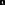
\includegraphics[width=\linewidth]{cho/kernel_final_5.png}
        \caption{5x5 estimation}
        \label{fig:h_cho_5}
    \end{subfigure}
    \hfill
    \begin{subfigure}[t]{0.14\textwidth}
        \centering
        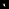
\includegraphics[width=\linewidth]{cho/kernel_final_7.png}
        \caption{7x7 estimation}
        \label{fig:h_cho_7}
    \end{subfigure}
    \hfill
    \begin{subfigure}[t]{0.16\textwidth}
        \centering
        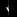
\includegraphics[width=\linewidth]{cho/kernel_final_9.png}
        \caption{9x9 estimation}
        \label{fig:h_cho_9}
    \end{subfigure}
    \hfill
        \begin{subfigure}[t]{0.18\textwidth}
        \centering
        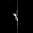
\includegraphics[width=\linewidth]{cho/kernel_final_11.png}
        \caption{11x11 estimation}
        \label{fig:h_cho_11}
    \end{subfigure}


    \caption{Evolution of the estimated kernels throughout Cho and Lee of the image shown in Fig \ref{fig:admm_progress}.}
    \label{fig:kernel_evolution}
\end{figure}




\subsection{Dictionary Reconstruction and the Results of the ADMM}


We use the predicted H and fix it throughout ADMM as a design choice. For the iterative steps of ADMM, initially we start with large dictionary constraint hyperparameter $\mu$ so that the estimated clear image update depends heavily on the dictionary reconstruction $\left\|z_x-D_z \alpha\right\|_2^2$, which promotes the iteration outcomes to lie in the clear image space (i.e which overall can be interpreted as avoidance of the trivial blurred prediction for the clear image, encouraged by the separate $h$ and $x$ optimization and dictionary reconstruction). The outcomes of the ADMM steps indicate the the predicted image gets cleared as steps increased as can be seen in Fig \ref{fig:admm_progress} and \ref{fig:admm_pipeline}. As can be seen on the Fig \ref{fig:skeleton_dict_results}, dictionary can reconstruct the clear image.




\begin{figure}[H]
    \centering

    % --- Input blur ---
    \begin{subfigure}[t]{0.32\textwidth}
        \centering
        \includegraphics[width=\linewidth]{skeleton\_dict/input\_blur\_1.png}
        \caption{Input blurred image}
        \label{fig:skeleton_input}
    \end{subfigure}
    \hfill
    % --- Dictionary reconstruction ---
    \begin{subfigure}[t]{0.32\textwidth}
        \centering
        \includegraphics[width=\linewidth]{skeleton\_dict/dict\_reconstruction\_19.png}
        \caption{Dictionary-based reconstruction}
        \label{fig:skeleton_dict_recon}
    \end{subfigure}
    \hfill
    % --- Final result ---
    \begin{subfigure}[t]{0.32\textwidth}
        \centering
        \includegraphics[width=\linewidth]{skeleton\_dict/final\_result\_1.png}
        \caption{Final deblurred result}
        \label{fig:skeleton_final}
    \end{subfigure}

    \caption{Deblurring using dictionary-based reconstruction on the building image.}
    \label{fig:skeleton_dict_results}
\end{figure}





\begin{figure}[!h]
    \centering

    % --- Row 1 ---
    \begin{subfigure}[t]{0.45\textwidth}
        \centering
        \includegraphics[width=\linewidth]{taha/admm/input\_blur.png}
        \caption{Blurred Input}
        \label{fig:admm_00}
    \end{subfigure}
    \hfill
    \begin{subfigure}[t]{0.45\textwidth}
        \centering
        \includegraphics[width=\linewidth]{taha/admm/admm\_03.png}
        \caption{ADMM iteration 3}
        \label{fig:admm_03}
    \end{subfigure}

    \vspace{0.4cm}

    % --- Row 2 ---
    \begin{subfigure}[t]{0.45\textwidth}
        \centering
        \includegraphics[width=\linewidth]{taha/admm/admm\_10.png}
        \caption{ADMM iteration 10}
        \label{fig:admm_10}
    \end{subfigure}
    \hfill
    \begin{subfigure}[t]{0.45\textwidth}
        \centering
        \includegraphics[width=\linewidth]{taha/admm/final\_result.png}
        \caption{Final ADMM result}
        \label{fig:admm_final}
    \end{subfigure}

    \caption{Evolution of the ADMM reconstruction across selected iterations and the final result.}
    \label{fig:admm_progress}
\end{figure}



\begin{figure}[!h]
    \centering

    % --- Row 1 ---
    \begin{subfigure}[t]{0.45\textwidth}
        \centering
        \includegraphics[width=\linewidth]{building/admm/input\_blur.png}
        \caption{Input blurred image}
        \label{fig:input_blur}
    \end{subfigure}
    \hfill
    \begin{subfigure}[t]{0.45\textwidth}
        \centering
        \includegraphics[width=\linewidth]{building/admm/admm\_03.png}
        \caption{ADMM iteration 3}
        \label{fig:admm_03_b}
    \end{subfigure}

    \vspace{0.4cm}

    % --- Row 2 ---
    \begin{subfigure}[t]{0.45\textwidth}
        \centering
        \includegraphics[width=\linewidth]{building/admm/admm\_10.png}
        \caption{ADMM iteration 10}
        \label{fig:admm_10_b}
    \end{subfigure}
    \hfill
    \begin{subfigure}[t]{0.45\textwidth}
        \centering
        \includegraphics[width=\linewidth]{building/admm/final\_result.png}
        \caption{Final ADMM reconstruction}
        \label{fig:final_result_b}
    \end{subfigure}

    \caption{ADMM deblurring process showing the input blurred image, intermediate reconstructions, and the final result.}
    \label{fig:admm_pipeline}
\end{figure}


We claim that the sharpness of the image can be measured by high frequency components and graident based metrics (such as Tenengrad $=\sum_{x, y}\left(G_x^2+G_y^2\right)$) and the metrics are shown in the Tables \ref{tab:metrics_table} and \ref{tab:metrics_table_eval}


\begin{table}[!h]
\centering
\caption{Sharpness-related metrics across ADMM iterations and final output (of Fig \ref{fig:admm_pipeline}).}
\label{tab:metrics_table}
\begin{tabular}{r l l r r r}
\toprule
\textbf{idx} & \textbf{label} & \textbf{file} & \textbf{grad\_power} & \textbf{tenengrad} & \textbf{hf\_ratio} \\
\midrule
0  & blur     & input\_blur.png     & 5.944804e-04 & 5.944804e-04 & 0.000861 \\
1  & admm\_00 & admm\_00.png        & 2.491733e-04 & 2.491733e-04 & 0.000255 \\
2  & admm\_01 & admm\_01.png        & 5.062831e-04 & 5.062831e-04 & 0.000146 \\
3  & admm\_02 & admm\_02.png        & 7.974522e-04 & 7.974522e-04 & 0.000214 \\
4  & admm\_03 & admm\_03.png        & 1.051128e-03 & 1.051128e-03 & 0.000313 \\
5  & admm\_04 & admm\_04.png        & 1.275241e-03 & 1.275241e-03 & 0.000442 \\
6  & admm\_05 & admm\_05.png        & 1.485745e-03 & 1.485745e-03 & 0.000598 \\
7  & admm\_06 & admm\_06.png        & 1.690356e-03 & 1.690356e-03 & 0.000786 \\
8  & admm\_07 & admm\_07.png        & 1.895307e-03 & 1.895307e-03 & 0.001009 \\
9  & admm\_08 & admm\_08.png        & 2.105915e-03 & 2.105915e-03 & 0.001276 \\
10 & admm\_09 & admm\_09.png        & 2.326757e-03 & 2.326757e-03 & 0.001605 \\
11 & admm\_10 & admm\_10.png        & 2.560284e-03 & 2.560284e-03 & 0.002021 \\
12 & admm\_11 & admm\_11.png        & 2.805360e-03 & 2.805360e-03 & 0.002558 \\
13 & admm\_12 & admm\_12.png        & 3.061679e-03 & 3.061679e-03 & 0.003263 \\
14 & admm\_13 & admm\_13.png        & 3.325560e-03 & 3.325560e-03 & 0.004183 \\
15 & admm\_14 & admm\_14.png        & 3.599105e-03 & 3.599105e-03 & 0.005386 \\
16 & admm\_15 & admm\_15.png        & 3.871754e-03 & 3.871754e-03 & 0.006822 \\
17 & admm\_16 & admm\_17.png        & 4.317180e-03 & 4.317180e-03 & 0.009264 \\
18 & admm\_17 & admm\_18.png        & 4.530648e-03 & 4.530648e-03 & 0.010648 \\
19 & admm\_18 & admm\_19.png        & 4.742994e-03 & 4.742994e-03 & 0.012195 \\
20 & final    & final\_result.png   & 4.742994e-03 & 4.742994e-03 & 0.012195 \\
\bottomrule
\end{tabular}
\end{table}



\begin{table}[!h]
\centering
\caption{Sharpness metrics computed over ADMM iterations and the final reconstructio (of Fig \ref{fig:admm_progress}) .}
\label{tab:metrics_table_eval}
\begin{tabular}{r l l r r r}
\toprule
\textbf{idx} & \textbf{label} & \textbf{file} &
\textbf{grad\_power} & \textbf{tenengrad} & \textbf{hf\_ratio} \\
\midrule
0  & blur     & input\_blur.png     & 5.694281e{-04} & 5.694281e{-04} & 0.000473 \\
1  & admm\_00 & admm\_00.png        & 3.109234e{-04} & 3.109234e{-04} & 0.000203 \\
2  & admm\_01 & admm\_01.png        & 6.035091e{-04} & 6.035091e{-04} & 0.000092 \\
3  & admm\_02 & admm\_02.png        & 9.359412e{-04} & 9.359412e{-04} & 0.000138 \\
4  & admm\_03 & admm\_03.png        & 1.230954e{-03} & 1.230954e{-03} & 0.000242 \\
5  & admm\_04 & admm\_04.png        & 1.482488e{-03} & 1.482488e{-03} & 0.000396 \\
6  & admm\_05 & admm\_05.png        & 1.683529e{-03} & 1.683529e{-03} & 0.000573 \\
7  & admm\_06 & admm\_06.png        & 1.862015e{-03} & 1.862015e{-03} & 0.000800 \\
8  & admm\_07 & admm\_07.png        & 2.027196e{-03} & 2.027196e{-03} & 0.001072 \\
9  & admm\_08 & admm\_08.png        & 2.186032e{-03} & 2.186032e{-03} & 0.001383 \\
10 & admm\_09 & admm\_09.png        & 2.339068e{-03} & 2.339068e{-03} & 0.001728 \\
11 & admm\_10 & admm\_10.png        & 2.481365e{-03} & 2.481365e{-03} & 0.002090 \\
12 & admm\_11 & admm\_11.png        & 2.609914e{-03} & 2.609914e{-03} & 0.002448 \\
13 & admm\_12 & admm\_12.png        & 2.723556e{-03} & 2.723556e{-03} & 0.002796 \\
14 & admm\_13 & admm\_13.png        & 2.822662e{-03} & 2.822662e{-03} & 0.003120 \\
15 & admm\_14 & admm\_14.png        & 2.908497e{-03} & 2.908497e{-03} & 0.003420 \\
16 & admm\_15 & admm\_15.png        & 2.981219e{-03} & 2.981219e{-03} & 0.003691 \\
17 & admm\_16 & admm\_16.png        & 3.044691e{-03} & 3.044691e{-03} & 0.003947 \\
18 & admm\_17 & admm\_17.png        & 3.103093e{-03} & 3.103093e{-03} & 0.004201 \\
19 & admm\_18 & admm\_18.png        & 3.157139e{-03} & 3.157139e{-03} & 0.004460 \\
20 & admm\_19 & admm\_19.png        & 3.209012e{-03} & 3.209012e{-03} & 0.004732 \\
21 & final    & final\_result.png   & 4.742994e{-03} & 4.742994e{-03} & 0.012195 \\
\bottomrule
\end{tabular}
\end{table}


Moreover, here is the radial FFT power plots to explicitly see how high frequencies are reintroduced after deblurring as can be seen in the Fig \ref{fig:radial_fft}.


\begin{figure}[H]
    \centering

    \begin{subfigure}[t]{0.45\textwidth}
        \centering
        \includegraphics[width=\linewidth]{taha/eval\_progress/radial\_fft\_overlay\_blur\_admm01\_admm05\_final.png}
        \caption{Cup}
        \label{fig:radial_fft_taha}
    \end{subfigure}
    \hfill
    \begin{subfigure}[t]{0.45\textwidth}
        \centering
        \includegraphics[width=\linewidth]{building/eval\_progress/radial\_fft\_overlay\_blur\_admm01\_admm05\_final.png}
        \caption{Building }
        \label{fig:radial_fft_building}
    \end{subfigure}

    \caption{Radial FFT comparison between the Cup and Building Images.}
    \label{fig:radial_fft}
\end{figure}

\subsection{Wiener vs ADMM}






We then compared visually the outputs of the baseline Wiener filter (using our estimated kernel to obtain the blur image.


As can be seen in the Fig \ref{fig:wiener_vs_admm} , the Wiener filter performs worse when it comes to especially 


\begin{figure}[!h]
    \centering

    \begin{subfigure}[t]{0.32\textwidth}
        \centering
        \includegraphics[width=\linewidth]{wiener-vs-admm/input\_blur.png}
        \caption{Input blurred image}
        \label{fig:wiener_admm_input}
    \end{subfigure}
    \hfill
    \begin{subfigure}[t]{0.32\textwidth}
        \centering
        \includegraphics[width=\linewidth]{wiener-vs-admm/deblur\_wiener.png}
        \caption{Wiener deblurring result}
        \label{fig:wiener_admm_wiener}
    \end{subfigure}
    \hfill
    \begin{subfigure}[t]{0.32\textwidth}
        \centering
        \includegraphics[width=\linewidth]{wiener-vs-admm/final\_result.png}
        \caption{ADMM deblurring result}
        \label{fig:wiener_admm_final}
    \end{subfigure}

    \caption{Comparison of input blur, Wiener deblurring, and ADMM-based deblurring.}
    \label{fig:wiener_vs_admm}
\end{figure}









\section{Discussion}


Our pipeline begins with kernel estimation, which is one of the most crucial part of the blind image de-blurring, since throughout our experiments, we have observed that the correct estimation of kernel affects the rest of the algorithms dramatically. In our method, we initialize the kernel in 5*5 dimensions, which appears to be engulfed by the motion blur (many white points), which can be avoided with larger size initialization. Nonetheless, Cho and Lee based approach fine tunes the kernel and clearly shows the alignment with the motion gradually. 


Based on our sharpness evaluation metrics, we clearly see that the  ADMM steps gradually increase sharpness as verified by the visual outputs too. Our learned patch-based dictionary shows its reconstruction capability. Moreover, experimented Wiener filter can under-perform our algorithm.

However, our algorithm ADMM is based on FFT domain to facilitate the updates, which implicitly assumes circular convolution model, which gives us wrap-around stripes at the edges. Additionally, adjusting the sweet-spot of the hyper-parameters is a lengthy process since our algorithm is slower due to many sub-steps such as dictionary learning, ISTA iterations inside the ADMM. Moreover, the performance depends highly on the dataset, from which we obtain the initialization of the kernel estimation and we learn the dictionary.













\section{Conclusion}

In this project, we aimed to address the deblurring of an image, by first estimating  the blur kernel via posterior sample initialization and multi-scale fine tuning, online patch dictionary learning for the sparse representation, indicating the clear image subspace and patch-wise ADMM iterative algorithm to gradually obtain the clear image. Hence, the method remains scalable to large datasets and high-resolution images. However, FFT wraps-around should be suppressed and the further fine tuning of various hyper-parameters to improve the performance of dictionary learning, ADMM and inside ISTA steps should be performed. This requires a lengthy careful fine tuning due to having many hyperparameter and longer ADMM iteration duration (when compared to classical Wiener). Initial kernel estimation and dictionary learning heavily rely on the utilized dataset. Thus, any non-ideal and incompatible dataset can give misleading results.

Although the entire algorithm requires to be further fine-tuned, the idea of learning a clear image subspace via Dictionary using as much dataset as we want and eventually turning our de-blurring task to an optimization problem with patch-wise feasible implementation builds the foundation of our project. Additionally, optimization based solution is about image restoration problem, agnostic to specific domains, this gives a solution for the cases outside the common de-blurring, as long as the dataset is available. 



\newpage


\section{Appendix}

\subsection*{Code Repository}

The codes and the full resolution file of this report are available at the following Google Drive folder:
\begin{center}
\url{https://drive.google.com/drive/folders/184Hr_ovZ_9c13t4jfxK1Y6azXnRJB092?usp=sharing}
\end{center}

Files included:
\begin{itemize}
    \item \texttt{Original Report File}
  \item \texttt{evaluate-metrics.py -> Performance metric evaluation}
  \item \texttt{Motion\_deblurring\_main\_code.py  -> Main algorithm}
  \item \texttt{wiener-test.py -> Wiener filtering using the estimated kernel for comparison purposes}
\end{itemize}









\newpage

\begin{thebibliography}{9}


\bibitem{ClassicBlur}
Wang, R., & Tao, D. (2014). Recent progress in image deblurring. arXiv preprint arXiv:1409.6838.


\bibitem{DeepBlur}
Zhang, K., Ren, W., Luo, W., Lai, W. S., Stenger, B., Yang, M. H., & Li, H. (2022). Deep image deblurring: A survey. International Journal of Computer Vision, 130(9), 2103-2130.





\bibitem{Levin-deblur}
Levin, A., Weiss, Y., Durand, F., & Freeman, W. T. (2009, June). Understanding and evaluating blind deconvolution algorithms. In 2009 IEEE conference on computer vision and pattern recognition (pp. 1964-1971). IEEE.

\bibitem{cho-fast}
Cho, S., & Lee, S. (2009). Fast motion deblurring. In ACM SIGGRAPH Asia 2009 papers (pp. 1-8).

\bibitem{OnlineDLearn}
Mairal, J., Bach, F., Ponce, J., & Sapiro, G. (2010). Online learning for matrix factorization and sparse coding. Journal of Machine Learning Research, 11(1).



\bibitem{D1}
Aleksey Alekseev (Kwentar). blur\_dataset [Data set]. GitHub. Available at: https://github.com/Kwentar/blur\_dataset



\bibitem{D2}
Bhalley, R. (n.d.). GoPro Deblur dataset [Data set]. Kaggle. 
https://www.kaggle.com/datasets/rahulbhalley/gopro-deblur


\bibitem{ADMM}
Afonso, M. V., Bioucas-Dias, J. M., & Figueiredo, M. A. (2010). Fast image recovery using variable splitting and constrained optimization. IEEE transactions on image processing, 19(9), 2345-2356.

\bibitem{ScaledADMM}
S.~Boyd, N.~Parikh, E.~Chu, B.~Peleato, and J.~Eckstein,
\newblock ``Distributed Optimization and Statistical Learning via the Alternating Direction Method of Multipliers,''
\newblock {\em Foundations and Trends in Machine Learning}, vol.~3, no.~1, pp.~1--122, 2011.

\bibitem{Circulant}
Gray, R. M. (2006). Toeplitz and circulant matrices: A review. Foundations and Trends in Communications and Information Theory, 2(3), 155–239.

\bibitem{FISTA}
Beck, A., & Teboulle, M. (2009). A fast iterative shrinkage-thresholding algorithm for linear inverse problems. SIAM journal on imaging sciences, 2(1), 183-202.

\bibitem{ISTA}

Daubechies, I., Defrise, M., & De Mol, C. (2004). An iterative thresholding algorithm for linear inverse problems with a sparsity constraint. Communications on Pure and Applied Mathematics: A Journal Issued by the Courant Institute of Mathematical Sciences, 57(11), 1413-1457.


\bibitem{Shan}
Shan, Q., Jia, J., & Agarwala, A. (2008). High-quality motion deblurring from a single image. Acm transactions on graphics (tog), 27(3), 1-10




\end{thebibliography}





\end{document}
